\documentclass[11pt, answers]{exam}
\renewcommand{\baselinestretch}{1.05}
\usepackage{amsmath,amsthm,verbatim,amssymb,amsfonts,amscd, graphicx}
\usepackage{graphics}

\usepackage{afterpage}
\usepackage{caption}

\usepackage{tikz}
\usepackage{fancybox}

\usepackage{clrscode3e}

\topmargin0.0cm
\headheight0.0cm
\headsep0.0cm
\oddsidemargin0.0cm
\textheight23.0cm
\textwidth16.5cm
\footskip1.0cm
\theoremstyle{plain}
\newtheorem{theorem}{Theorem}
\newtheorem{corollary}{Corollary}
\newtheorem{lemma}{Lemma}
\newtheorem{proposition}{Proposition}
\newtheorem*{surfacecor}{Corollary 1}
\newtheorem{conjecture}{Conjecture}  
\theoremstyle{definition}
\newtheorem{definition}{Definition}

 \begin{document}
 


\title{CSC263: Assignment 2}
\date{February 9th, 2017}
\author{Junjie Cheng, Jiayun Liu, Zi Hao Lin}
\maketitle

\unframedsolutions

%Question2
\begin{solution}
\begin{parts}
\part 

Disprove: \\
Let T be: \\
\begin{minipage}[t]{\linewidth}
                \centering
\begin{tikzpicture}
[ 
level distance=9mm, 
every node/.style={circle, draw, inner sep=1.5pt},
level 1/.style={sibling distance=22mm}, 
level 2/.style={sibling distance=10mm}, 
label distance=-1mm
]

\node (root) [label=90:$+1$] {7} 
child {node[label=90:$0$] {3} 
    child{missing}
    child{missing}
}
child {node[label=90:$-1$] {11}
 	child {node[label=90:$0$] {9} 
 	}
    child {missing}
};
\end{tikzpicture}
\end{minipage}

Let $T'= delete(T,3)$ be: \\
\begin{minipage}[t]{\linewidth}
                \centering
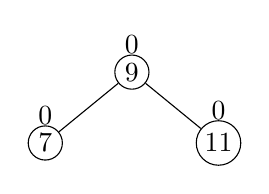
\begin{tikzpicture}
[ 
level distance=9mm, 
every node/.style={circle, draw, inner sep=1.5pt},
level 1/.style={sibling distance=22mm}, 
level 2/.style={sibling distance=10mm}, 
label distance=-1mm
]

\node (root) [label=90:$0$] {9} 
child {node[label=90:$0$] {7} 
}
child {node[label=90:$0$] {11}
};
\end{tikzpicture}
\end{minipage}

Let $T''= insert(T',3)$ be: \\
\begin{minipage}[t]{\linewidth}
                \centering
\begin{tikzpicture}
[ 
level distance=9mm, 
every node/.style={circle, draw, inner sep=1.5pt},
level 1/.style={sibling distance=22mm}, 
level 2/.style={sibling distance=10mm}, 
label distance=-1mm
]

\node (root) [label=90:$-1$] {9} 
child {node[label=90:$-1$] {7} 
    child{node[label=90:$0$] {3}}
    child {missing}
}
child {node[label=90:$0$] {11}
 	child {missing}
    child {missing}
};
\end{tikzpicture}
\end{minipage}

Then $T'' \neq T$.\\

\part
Suppose T is a tree with 12 nodes:\\
\begin{minipage}[t]{\linewidth}
                \centering
\begin{tikzpicture}
[ 
level distance=9mm, 
every node/.style={circle, draw, inner sep=1.5pt},
level 1/.style={sibling distance=45mm}, 
level 2/.style={sibling distance=22mm}, 
level 3/.style={sibling distance=10mm},
level 4/.style={sibling distance=7mm},
label distance=-1mm
]

\node (root) [label=90:$-1$] {8} 
child {node[label=130:$-1$] {5} 
	child {node[label=130:$-1$] {3} 
		child {node[label=130:$-1$] {2}
		    child {node[label=130:$0$] {1}} 
		    child {missing}} 
		child {node[label=130:$0$] {4}} 
	}
	child {node[label=50:$-1$] {7} 
		child {node[label=130:$0$] {6}} 
		child{missing}
	} 
}
child {node[label=50:$-1$] {11}
 	child {node[label=130:$-1$] {10}
 	    child{node[label=130:$0$] {9}}
 	    child{missing}}
 	child {node[label=50:$0$] {12}	}
};
\end{tikzpicture}
\end{minipage}

Then when we do $delete(T,12)$ First rebalancing:\\
\begin{minipage}[t]{\linewidth}
                \centering
\begin{tikzpicture}
[ 
level distance=9mm, 
every node/.style={circle, draw, inner sep=1.5pt},
level 1/.style={sibling distance=45mm}, 
level 2/.style={sibling distance=22mm}, 
level 3/.style={sibling distance=10mm},
level 4/.style={sibling distance=7mm},
label distance=-1mm
]

\node (root) [label=90:$-2$] {8} 
child {node[label=130:$-1$] {5} 
	child {node[label=130:$-1$] {3} 
		child {node[label=130:$-1$] {2}
		    child {node[label=130:$0$] {1}} 
		    child {missing}} 
		child {node[label=130:$0$] {4}} 
	}
	child {node[label=50:$-1$] {7} 
		child {node[label=130:$0$] {6}} 
		child{missing}
	} 
}
child {node[label=50:$0$] {10}
 	child {node[label=130:$0$] {9}}
 	child {node[label=50:$0$] {11}	}
};
\end{tikzpicture}
\end{minipage}

But now the right sub-tree is shorter, so we need a second rebalancing:\\
\begin{minipage}[t]{\linewidth}
                \centering
\begin{tikzpicture}
[ 
level distance=9mm, 
every node/.style={circle, draw, inner sep=1.5pt},
level 1/.style={sibling distance=45mm}, 
level 2/.style={sibling distance=22mm}, 
level 3/.style={sibling distance=10mm},
level 4/.style={sibling distance=7mm},
label distance=-1mm
]

\node (root) [label=90:$0$] {5} 
child {node[label=130:$-1$] {3} 
	child {node[label=130:$-1$] {2} 
		child {node[label=130:$0$] {1}}
		child {missing} 
	}
	child {node[label=50:$0$] {4} 
		child{missing} 
		child{missing}
	} 
}
child {node[label=50:$0$] {8}
 	child {node[label=130:$-1$] {7}
 	    child{node[label=130:$0$] {6}}
 	    child{missing}}
 	child {node[label=50:$0$] {10}
 	    child{node[label=50:$0$] {9}}
 	    child{node[label=50:$0$] {11}}}
};
\end{tikzpicture}
\end{minipage}

\end{parts}
\end{solution}
\end{document}

